


\chapter{Marco teórico}
\label{ch:marco}

%%%%%%%%%%%%%%%%%%%%%%%%%%%%%%%%%%%%%%%%%%%%%%%%%%%%%%%%%%%%%%%%%%%%%%%%%%%%%%%%%%%%%%%%%%%%%
\section{Lógica Reconfigurable}

En 1991 nace comercialmente la primera computadora reconfigu
rable, la Algotronix CHS2X4. Previo a este hito, la investigación respectiva a la lógica
reconfigurable data a la década de 1960 donde Gerald Estrin propuso el concepto pio
nero de una computadora con una matriz reconfigurable de hardware, donde su uso se
adapta a la necesidad y una vez terminado su objetivo se podría darle propósito con
un nuevo objetivo. Posteriormente surgieron investigaciones destacables con arquitectu
ras reconfigurables como Copacabana, Matrix, GARP, Elixent, NGEN, Polyp, MereGen,
PACT, XPP, Silicon Hive, Montium, Pléyades, Morphosys y PiCoGA, cabe mencionar
que la convergencia ante la investigación de las lógica reconfigurable y sus posibles ar
quitecturas es una consecuencia del creciente mercado del silicio en los años ochentas y
noventas. La idea era efectiva, una pieza de hardware que mediante el software se le pu
diese cambiar el funcionamiento, así es como se originan los lenguajes de descripción de
hardware. Los lenguajes de descripción de hardware surgen de la idea de simplificar la
programación de las arquitecturas reconfigurables, se puede expresar su funcionamiento
mediante la descripción del sistema basado en sus entradas, salidas, reiteraciones y fun
ciones lógicas/aritméticas.  La descripción de hardware da rienda a múltiples niveles de
abstracción para generar la misma celda lógica, desde el uso de un operador aritmético,
por su construcción mediante compuertas lógicas o su diseño en el nivel de abstracción de
celda. Estos niveles de abstracción permiten simplificar el diseño del software de manera
que no es necesario describir las conexiones físicas a las compuertas, permitiendo que con
la descripción de su funcionamiento el sistema funcione sin la necesidad de explicar sus
conexiones internas. Luego de la síntesis del software se espera que entre menor sea el
nivel de abstracción utilizado, se minimice al pasarlo al hardware, por lo que la com
plejidad a nivel de compuertas será mayor que a nivel funcional. Algunos ejemplos de
lenguajes de descripción de hardware son VHDL, Verilog, System Verilog, Slide, Conlan,
ISPS, Adlib, Hill, Oode y Boris. La jerarquía del diseño dicta el orden de funcionamiento
de los múltiples diseños que pueden ser utilizados por otro diseños, por lo que contar
con un diseño básico como una compuerta “and” y que esta tenga una jerarquía superior
al diseño que la va a utilizar generar un problema de jerarquías ya que el diseño que la
iba a utilizar no puede encontrarla. Esta característica de los lenguajes de descripción
de hardware permite la escalabilidad y modularización de sistemas extensos, en lugar de
describir un procesador se pueden describir sus partes y mediante la jerarquía se realiza
un diseño superior que una las partes del mismo, de igual manera permite la revisión de
todos los componentes para el buen desarrollo del sistema.
\cite{hassani2024efficient, kuon2007fpga, meyerbaese2014digital} 


\section{Arquitectura interna de FPGAs}

Las FPGAs como su nombre en inglés las describen son Arreglos de compuertas lógicas
programables, por lo que su arquitectura se basa en matrices de bloques lógicos, conmuta
ciones para el direccionamiento de los datos y el enrutamiento, en la figura 2.1 se observa
un diagrama simplificado de la arquitectura interna de una FPGA simple.
\cite{hassani2024efficient, kuon2007fpga, meyerbaese2014digital} 

\begin{figure}[h!]
    \centering 
    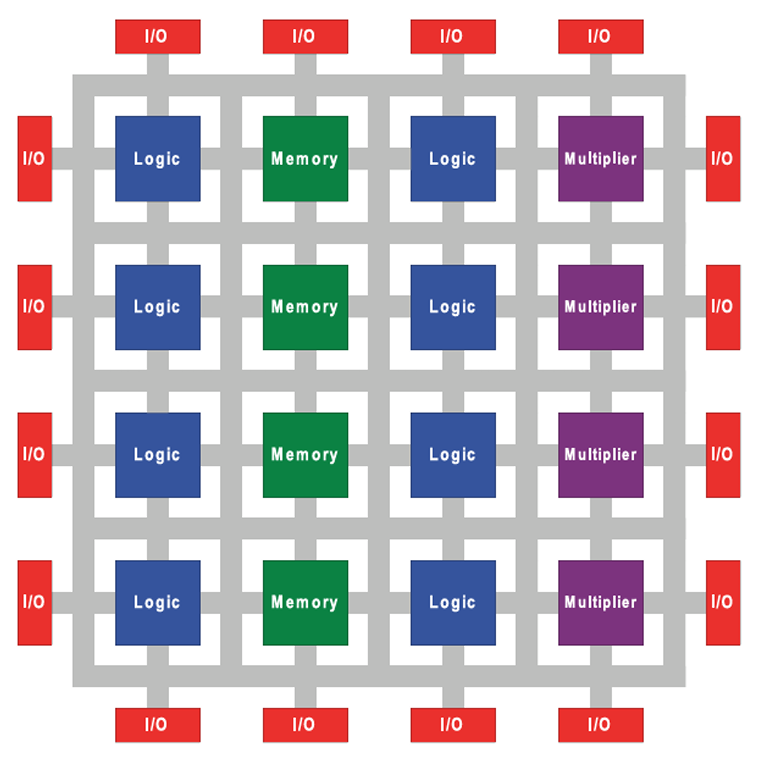
\includegraphics[width=0.6\linewidth]{pics/Uno.png} 
    \caption{Diagrama simplificado de matriz de programable de compuertas lógicas. \cite{kuon2007fpga}}
    \label{fig:Uno} 
\end{figure}

\subsection{Tablas de Consulta}

Las tablas de consulta son la herramienta mediante la cual se genera la lógica en una
FPGA, en lugar de utilizar compuertas lógicas y tener que redirigir miles de compuertas
lógicas, lo que se utiliza son celdas de memoria en conjunto con multiplexores de esta
manera se genera una tabla de verdad dentro del sistema mediante un bitstream que lo
configura. También son conocidas como LUTs, según la cantidad de entradas se le añade
un número al final a modo de identificación, del número de entradas depende la cantidad
de bits de configuración que tiene una LUT en el caso de una LUT4 se tienen 16 posiciones
de memoria para cada una de las cuatro entradas y para la salida, en el caso de una LUT6
se tiene 64 bits de configuración. Aunque las LUTs sean escalables es importante analizar
las consecuencias de su escalabilidad, ya que existe una curva que describe los cambios en
el área y cantidad de LUTs en cierto área.
\cite{hassani2024efficient, kuon2007fpga, meyerbaese2014digital} 

En la figura 2.2 se muestra que el punto óptimo del tamaño de las LUTs se encuentra cerca
de LUT5, no obstante, se aclara que esto no impide tener LUT6 aunque solo se cuente
con LUT5, debido a que se va a trabajar con conglomerados de LUTs estos se pueden
conectar en paralelo para crear LUTs modulares que representen un LUT6, a forma de
ejemplo los LUT5 tienen 32 posiciones de memoria y los LUT6 tienen 64 posiciones de
memoria, por lo que al utilizar dos LUT5 se puede generar la lógica necesaria para un
LUT6. La práctica anterior es una eficiente solución para evitar el malgasto de área de la
FPGA enLUTs. Anivel de implementación física se suele utilizar SRAM para la memoria
de las LUTs y estos constituyen los bloques blandos de la FPGA.
\cite{kuon2007fpga, abderrahmaneMaximizeFlexibility}

\begin{figure}[h!]
    \centering 
    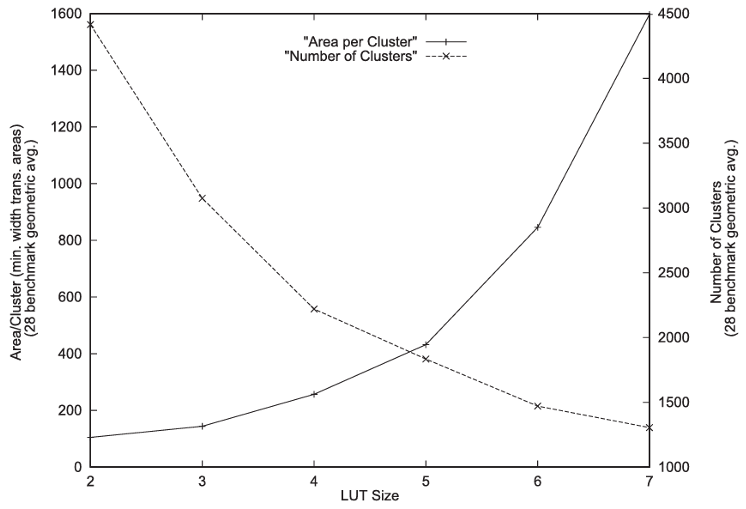
\includegraphics[width=0.7\linewidth]{pics/Dos.png} 
    \caption{Grafica de LUT de uso optimo. \cite{kuon2007fpga}}
    \label{fig:Dos} 
\end{figure}


Se debe tomar en cuenta para la eficiencia de una FPGA, no solo tiene lógica reconfigu
rable, también cuenta con módulos especializados, en el caso de que toda la lógica sea
reconfigurable, se pueden utilizar múltiples LUTs en algo que no es necesario por ejemplo
en bloques de multiplicación, este tipo de bloque es conocido como bloque rígido ya que
su función es fija. Su implementación es grabada sobre el propio silicio haciéndola no
reconfigurable, pero su ventaja se encuentra en su rendimiento ya que al estar sobre el
silicio funcionan de manera más rápida que una tabla de consulta y requiere poca área
del silicio.
\cite{kuon2007fpga, meyerbaese2014digital, abderrahmaneMaximizeFlexibility}

\subsection{Enrutamiento}

La arquitectura del enrutamiento en una FPGA es lo que da conexión a las LUTs al
igual que sus entradas, salidas y los bloques rígidos para completar la lógica diseñada. La
arquitectura utilizada es la arquitectura tipo isla como se muestra en la figura 2.3. En
dicha arquitectura se tienen los bloques lógicos y canales de enrutamiento a los cuatro
lados de dichos bloques lógicos, la cantidad n de cables que contiene un canal se define
durante la fabricación, sin embargo, es de los parámetros más importantes que puede
tener una FPGA ya que define la cantidad de señales que se pueden trabajar de manera
simultánea.
\cite{hassani2024efficient, kuon2007fpga} 

\begin{figure}[h!]
    \centering 
    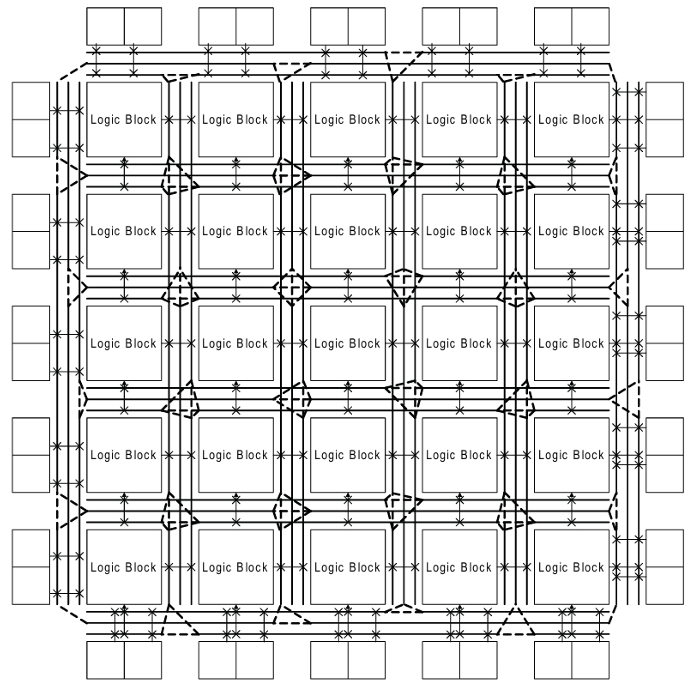
\includegraphics[width=0.6\linewidth]{pics/Tres.png} 
    \caption{Diagrama de configuración del enrutamiento y bloques lógicos. \cite{kuon2007fpga}}
    \label{fig:Tres} 
\end{figure}


La lógica de la arquitectura de isla se basa en dos sencillos términos, cables largos y
cables cortos, los cables largos componen los canales que se observan en paralelo a los
bloques lógicos, su principal función es ser una malla de interconexión entre las señales
que se generen o ingresen a la FPGA. Los cables cortos son el medio por el que las señales
entran a un bloque desde la malla de enrutamiento o por la que la señal sale de un bloque
a la malla de enrutamiento como se muestra en la figura 2.4.
 \cite{kuon2007fpga, meyerbaese2014digital} 

\begin{figure}[h!]
    \centering 
    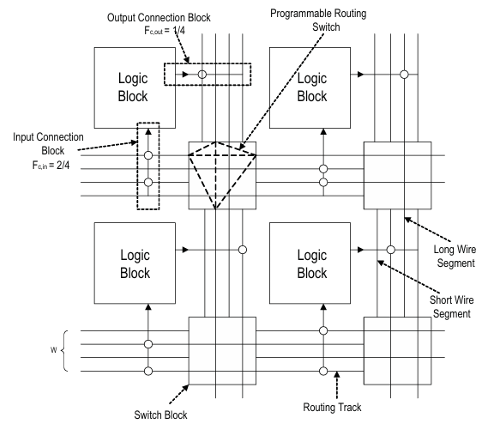
\includegraphics[width=0.6\linewidth]{pics/Cuatro.png} 
    \caption{Diagrama de bloques de cables cortos y largos. \cite{kuon2007fpga}}
    \label{fig:Cuatro} 
\end{figure}


Cabe mencionar que existen arquitecturas de enrutamiento que dependen del orden jerárquico 
para ordenar la transferencia de datos, pero a manera que la jerarquía aumenta, los
retardos aumentan de manera significativa perdiendo el sentido de que existan múltiples
niveles jerárquicos y haciendo esta arquitectura contraproducente al objetivo de flexibili
dad inherente de una FPGA. La malla de enrutamiento se encarga del desplazamiento de
datos en la arquitectura de una FPGA, no obstante, la gestión de los datos es responsa
bilidad de la matriz de conmutación.
\cite{hassani2024efficient, kuon2007fpga} 

\subsection{Matriz de conmutación}

La malla de enrutamiento conecta todos los bloques de la arquitectura, pero aún se deben
dirigir dichos datos, para que sean la entrada de un bloque o inclusive para que dos bloques
trabajen los datos en paralelo, la matriz de conmutación es el mecanismo mediante el cual
se ordenan las pistas de cables y se define a las señales cuál bloque es su próximo ingreso.
Estas rutas se definen desde que se carga el bitstream a la FPGA, por lo que las rutas
son flexibles previas al bitstream, pero estáticas una vez programadas. Su funcionamiento
se caracteriza por el uso de multiplexores para definir la ruta, sin embargo también se
implementa la lógica necesaria mediante transistores de paso para definir su ruta.
\cite{hassani2024efficient, kuon2007fpga} 

Se considera la intersección de dos canales como una matriz de conmutación, en dichos
canales donde cada cable interseca con otro cable se debe considerar la posibilidad de que
la señal viaje sobre el mismo cable en la misma dirección inicial, que siga una ruta ascen
dente por el cable con el que interseca, o una ruta descendente por el cable que interseca.
Para definir la ruta específica que se desea, se requieren de al menos seis transistores de
paso para aislar la ruta en el caso de que no se desee bifurcar la señal, las ubicaciones
específicas para dichos transistores de paso son conectando la sección de cable izquierdo
con el derecho, conectando la sección ascendente con la descendente, la izquierda con la
ascendente, la izquierda con la descendente, la ascendente con la derecha y la descendente
con la derecha, de esta manera se tiene un control total sobre la dirección deseada de la
señal, su control se basa en los datos guardados en una memoria SRAM que requiere seis
bits de control, considerando un bit por transistor de paso y una SRAM por intersección
de los cables largos tal y como se muestra en la figura número.
\cite{hassani2024efficient, kuon2007fpga} 

\begin{figure}[h!]
    \centering 
    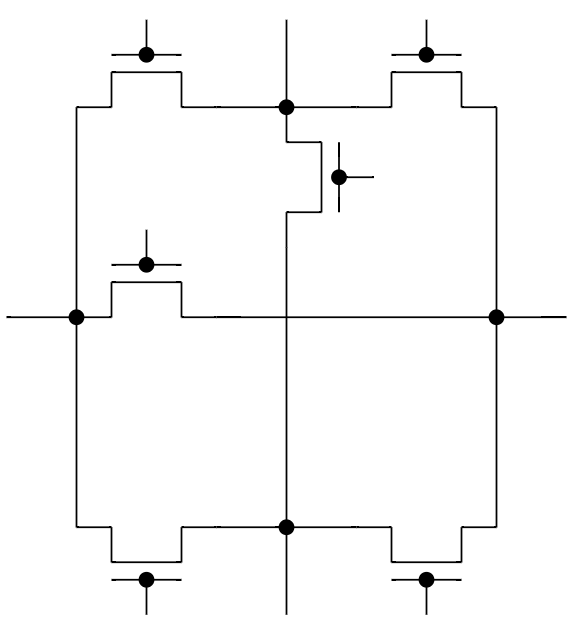
\includegraphics[width=0.4\linewidth]{pics/Cinco.png} 
    \caption{Diagrama matriz de conmutación.  \cite{kuon2007fpga}}
    \label{fig:Cinco} 
\end{figure}

\section{Arquitectura Modulo de Jerarquía Superior}

Considerando el funcionamiento de una FPGA, es necesario tener un conocimiento del
proceso entre el diseño y la descripción de hardware, para cualquier sistema, esto debido
al flujo de bits necesario para dar propósito a la FPGA. Se debe implementar un inyector
del flujo de bits además de la FPGA embebida en el nivel superior de jerarquía, de otra
manera la FPGA embebida se mantiene en un estado sin programar. Se requiere algún tipo
de memoria que se pueda utilizar para luego serializar y cargarla a la FPGA embebida.
Las ROM cumplen con características específicas para probar el funcionamiento de la FP
GAembebida en conjunto con lógica secuencial que permite la serialización de los datos de
la ROM para su posterior inyección en el sistema, de esta implementación suele encargarse
el software de diseño en conjunto con los puertos del hardware para la configuración.
\cite{hassani2024efficient, kuon2007fpga, meyerbaese2014digital} 

\subsection{Escaneo de Fronteras/JTAG}
El Joint Test Action Group, fue desarrollado para resolver problemas en el área de testing 
de circuitos integrados, esto debido a que los circuitos integrados cada vez disminuían el 
tamaño y los pines de prueba que se utilizaban acaparaban mucha área del circuito integrado 
por lo que se investigaban nuevos métodos de probar la funcionalidad de los circuitos 
integrados. El estándar IEEE 1149.1 surge en 1990 y define la arquitectura TAP en conjunto 
con el JTAG para diagnóstico, manufactura, validación, caracterización y debug de los 
circuitos integrados. 
\cite{nelsonBoundaryScan, calvoTestingSesion4, xjtagWhatIsJtag, jtagTechnologiesBoundaryScan, jtagTechnologiesTapController, ieee1149}

\begin{figure}[h!]
    \centering 
    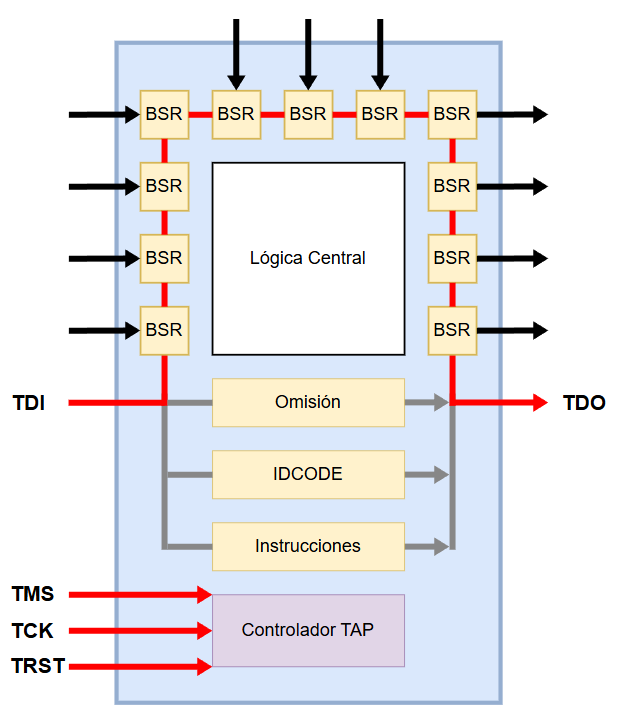
\includegraphics[width=0.4\linewidth]{pics/Seis.png} 
    \caption{Diagrama de la arquitectura TAP. \cite{jtagTechnologiesBoundaryScan}}
    \label{fig:Seis} 
\end{figure}

\subsection{Interfaz del Puerto de Acceso de Prueba}

Su conexión física se basa en 4 pines, TDI (Entrada de datos serial), TMS (Control), TCK (Reloj), 
TDO (Salida de datos serial) y en ocasiones se añade un pin extra TRST (Reinicio asíncrónico), estas cuatro o 
cinco señales son conocidas como TAP (Puertos de acceso para pruebas). En el contexto de las 
FPGAs , se utiliza el JTAG para acceder a la configuración de la memoria para programar el 
dispositivo, para visualizar la lógica programable del núcleo y el ruteo de los recursos. 
Esto se ejemplifica en las secciones pasadas dedicadas a explicar la arquitectura de lógica 
reconfigurable de las FPGAs, donde los registros SRAM configuran las tablas de búsqueda, los 
caminos que deben seguir los recursos y la disposición de la matrices de conmutación.
\cite{nelsonBoundaryScan, calvoTestingSesion4, jtagTechnologiesBoundaryScan, jtagTechnologiesTapController} \cite{ieee1149}

\begin{figure}[h!]
    \centering 
    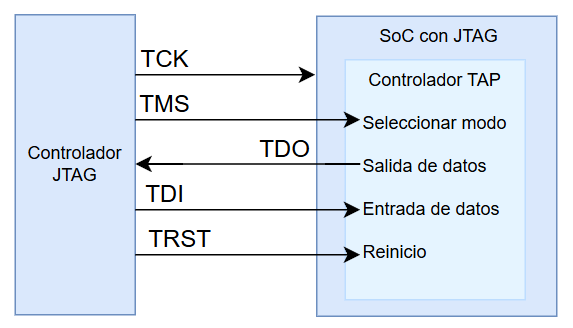
\includegraphics[width=0.6\linewidth]{pics/Siete.png} 
    \caption{Diagrama de conexion JTAG y TAP.  \cite{jtagTechnologiesTapController}}
    \label{fig:Siete} 
\end{figure}


\subsection{Controlador JTAG TAP}

El controlador TAP es el mecanismo de control base del estándar IEEE 1149.1, en este se 
define como los datos son ciclados a través del dispositivo y determina si se accede a alguno 
de los registris de datos e/o instruciones. Las señales del controlador se acceden mediante 
la interfaz TAP explicada anteriormente. El pin de mayor significado para el codntrolador TAP 
es el TMS debido a que es la entrada (un solo bit) de la máquina de estados que define el 
camino a tomar de los 16 estados existentes.
\cite{nelsonBoundaryScan, calvoTestingSesion4, jtagTechnologiesBoundaryScan, jtagTechnologiesTapController, ieee1149}

Al ordenar los estados en funcionalidad, se obtinen 3 subcategorías:
\begin{itemize}
    \item Prueba de lógica de reinicio y Marcha/Inactivo.
    \item Estados de accedo al registro de insrucciones (IR).
    \item Estados de acceso a los registros de datos (DR).
\end{itemize}
\cite{nelsonBoundaryScan, calvoTestingSesion4, jtagTechnologiesBoundaryScan, jtagTechnologiesTapController, ieee1149}

\begin{figure}[h!]
    \centering 
    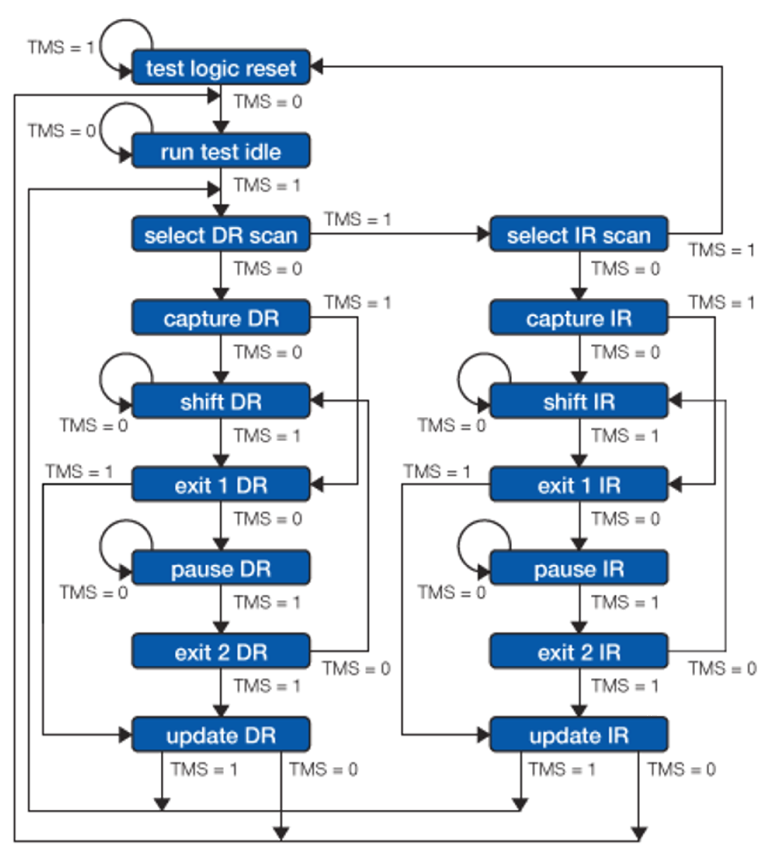
\includegraphics[width=0.6\linewidth]{pics/Ocho.png} 
    \caption{Máquina de estados del controlador TAP.  \cite{jtagTechnologiesTapController}}
    \label{fig:Ocho} 
\end{figure}

\subsection{Registros del JTAG}

El estándar IEEE 1149.1 define dos tipos de registros, los registros de datos y los registros 
de instrucciones. 
\cite{nelsonBoundaryScan, calvoTestingSesion4, jtagTechnologiesBoundaryScan, jtagTechnologiesTapController, ieee1149}

\subsubsection{Registros de datos}
Los registros de datos incluyen:

\begin{itemize}
    \item El registro de escaneo de frontera (BSR).
    \item El registro de omisión (BYPASS).
    \item El registro del código de identificación (IDCODE).
\end{itemize}

El controlador TAP se encarga de definir a cuál se accesa mediante la máquina de estados ya 
que solo se puede utilizar un registro de datos a la vez. 
\cite{nelsonBoundaryScan, calvoTestingSesion4, jtagTechnologiesBoundaryScan, jtagTechnologiesTapController, ieee1149}

El BSR no es un registro de un solo bloque, sino el una cadena de bloques que funcioan como 
registro de corrimiento para forzar valores a pines específicos internamente en el SoC, de 
igual manera se puede utilizar como un muestreo  de los valores de los pines considerando que 
son solo de lectura para realizar un censado.
\cite{nelsonBoundaryScan, calvoTestingSesion4, jtagTechnologiesBoundaryScan, jtagTechnologiesTapController, ieee1149}

El registro de omisión solo cuenta con un bit de logitud, y su función es habilitar o 
desconectar el uso del registro BSR, funciona como paso a la entrada de otros SoC que se 
quieren probar en serie con el primero, esto permite la optimización del flujo de bits.  
\cite{nelsonBoundaryScan, calvoTestingSesion4, jtagTechnologiesBoundaryScan, jtagTechnologiesTapController, ieee1149}

El registro del código de identificación es un registro de 32 bits que contiene la 
identificación única del dispositivo, está grabada en el silicio para evitar su modificación, 
sirve para que el software sea capaz de identificar el hardware y utilice valores correctos de 
tensión para el registro BSR y la correcta cantidad de bits.
\cite{nelsonBoundaryScan, calvoTestingSesion4, jtagTechnologiesBoundaryScan, jtagTechnologiesTapController, ieee1149}

\section{Filtrado digital}

Basado en la funcionalidad de la transformada discreta de Fourier como representación
finita en el dominio de la frecuencia. El filtro digital es un filtro matemático que realiza
una convolución, que matemáticamente se puede explicar secuencialmente como un des
plazamiento temporal, la multiplicación de la señal por otra señal de referencia y la suma
de los resultados para generar el muestreo de la salida. Los filtro digitales se dividen en
dos tipos:
\begin{itemize}

    \item Filtros digitales de respuesta finita al impulso: Estos filtros tienen una respuesta
finita al impulso, lo que significa que su salida se vuelve cero después de un número
finito de muestras. Son estables y tienen una fase lineal, lo que los hace ideales para
aplicaciones donde la distorsión de fase es un problema.\cite{proakis1996digital}

    \item Filtros digitales de respuesta infinita al impulso: Estos filtros tienen una respuesta
infinita al impulso, lo que significa que su salida no se vuelve cero después de un
número finito de muestras. Son más eficientes en términos de recursos computacio
nales, pero pueden ser inestables y tener una fase no lineal.\cite{proakis1996digital}

\end{itemize}

Un ejemplo de un tipo de filtro digital es el filtro de coseno alzado, utiliza como referencia
un coseno y su principal fortaleza es reducir la interferencia entre símbolosonfiabilidad de
la transmisión de datos. El filtro de coseno alzado se utiliza en sistemas de comunicación
digital donde los símbolos pueden superponerse debido a la dispersión del canal.
\cite{proakis1996digital}

\section{Estado del Arte}

\subsection{eFPGAs}

El concepto de una FPGA embebida no es nuevo, las FPGAs se utilizan como solución an
tes piezas de hardware caras cuyo diseño no es complejo a nivel de características como la
potencia requerida o almacenamiento significativo. Su uso se encuentra incluso vinculado
a ASICs ya que también significa ahorro para los productores de dicho ASIC, no obstante,
en casos de eFPGAs en ASICs, las eFPGAs cuentan con características específicas para
la pieza de hardware que se desea implementar en conjunto con el ASIC, por lo que no se
espera una gran cantidad de tablas de consulta, menores velocidades de reloj para lógica
secuencial, e incluso puede que no se cuente con bloques rígidos especializados a menos
que el ASIC lo requiera. Algunos ejemplos de empresas a continuación.\cite{saidi2018survey}

Flex Logic es una compañía tecnológica que utiliza la tecnología de eFPGA desde el 2015,
los motiva la reutilización de un circuito integrado luego de su fabricación. Cuentan con
un núcleo de eFPGA conocido como FLX10 con 5-7 capas de metal, sus características
principales son:

\begin{itemize}

    \item 20K bits de RAM
    \item 122500 LUTs 6
    \item Coarse Grain
    
\end{itemize}

Mental trabaja con eFPGA desde el 2009, al igual que Flex Logic su objetivo es la
modificación de hardware post producción. La eFPGA de Menta cuenta con sus propias
herramientas para la compilación, diseño en RTL y configuración del eFPGA llamada
Origami.\cite{saidi2018survey}

\begin{itemize}

    \item 200000 LUTs 4
    \item Fine Grain
    
\end{itemize}

Achronix trabaja con eFPGA desde el 2016 su modelo de Speedcore eFPGA inlcuye
bloques de RAM, y bloques de procesamiento de señales digitales. Cuenta con el software
ACE para el diseño de herramientas, su principal uso es como acelerador de hardware y
coprocesador reconfigurable.\cite{saidi2018survey}

\begin{itemize}

    \item 1000 LUTs
    \item Coarse Grain
    
\end{itemize}

NanoXplore es una compañía que data del 2014 cuenta con la eFPGA NX-eFPGA que
se puede configurar mediante la aplicación NanoXmap para sintetizar RTL hasta el flujo
de bits, el uso de tablas de consulta de 4 entradas le permite utilizar menor área para la
eFPGA en la ASIC predeterminada.\cite{saidi2018survey}

\begin{itemize}

    \item 750000 LUTs
    \item Coarse Grain
    
\end{itemize}

La academia también presenta varias arquitecturas de eFPGA entre ellas:

\begin{itemize}
    \item FASE eFPGA
    \item EFPGA Based on Multistage Switching Networks
    \item ACLBs eFPGA
    \item Overlay eFPGA
    \item EFPGAs based on a flexible architecture
    \item ESL Re-programmable eFPGA
    \item EFPGA Subsystem
    \item LIP6 eFPGA
    \item FlexTiles
\end{itemize}

No se detallan sus características debido a que la mayoría utiliza LUTs de entre 4 y
6 entradas. Su uso es similar, sustituir una ASIC costosa en la implementación de un
proyecto o para investigación de su desarrollo.\cite{saidi2018survey}

\subsection{Herramientas de software}

FABulous es un generador de FPGA de código libre que implementa herramientas como
Yosys y nextpnr para el flujo de diseño, cuenta con la licencia Apache 2.0 para uso
comercial y académico. Cuenta con cierre del diseño de TSMC de 180nm, Skywater dde
130nm, IHP SG13G2, GF180MCU y 28nm CMOS.\cite{fabulous2024}

Yosys es una herramienta de código abierto para síntesis de Verilog RTL, tiene la licencia
ISC.\cite{wolf2024yosys}

\begin{itemize}

    \item Procesa casi cualquier diseño sintetizable en Verilog-2005.
    \item Mapeo a librerías de celdas estándar para ASICs.
    \item Mapeo para FPGAs Xilinx Serie 7 y Lattice iCE40 y ECP5.
    
\end{itemize}

Openlane es un traductor de RTL a GDSII basado en múltiples componentes como Yosys,
Magic, Netgen, CVC, SPEF-Extractor, Kayout entre otros, y es de código abierto. \cite{openlane}

%%%%%%%%%%%%%%%%%